\chapter{Periodic Boundary Conditions}

\graphicspath{{./Figures/PBC/}}

\section{Introduction}
Earlier sections described how quantum chemical techniques can be used
to determine the electronic structure of molecules. In addition to
molecules, we would also like to be able to describe systems like
polymers, surfaces, and crystals, where a simple \emph{unit cell} is
replicated periodically in 1, 2, or 3 dimensions. A sample unit cell
configuration is shown in Figure \ref{lattice-vectors}. This section
will survey the techniques used to describe systems with periodic
boundary conditions.

\begin{figure}
\begin{center}
\includegraphics{lattice-vectors.eps}
\caption{Lattice vectors (\matvec{b_1},\matvec{b_2},\matvec{b_3}) that
define the unit cell in a periodic solid.}
\label{lattice-vectors}
\end{center}
\end{figure}

\section{Energy Bands}
We know from our earlier studies that when we use quantum mechanics to
atoms or molecules we obtain a discrete set of states. Solids contain
on the order of $10^{23}$ atoms, and consequently these discrete
states are blurred into \emph{bands}.

\begin{figure}
\begin{center}
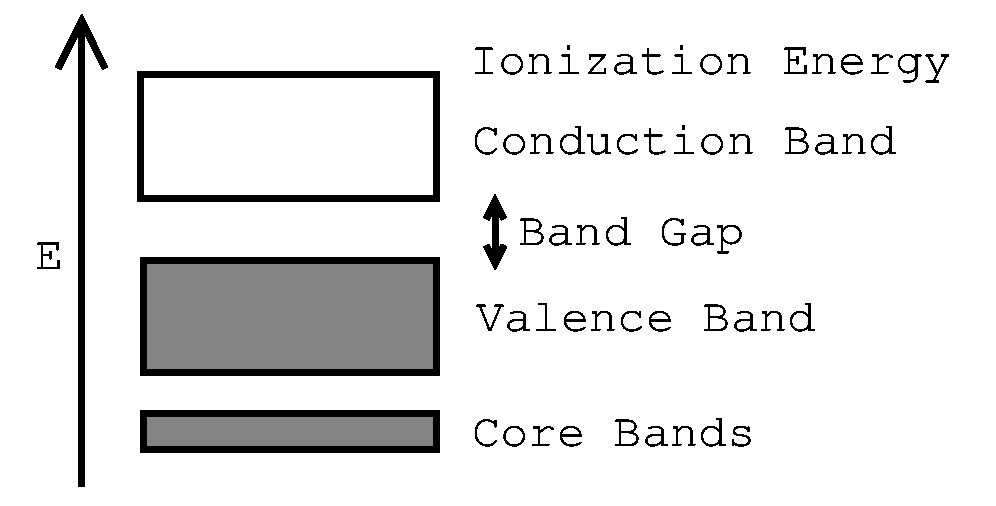
\includegraphics[scale=0.5]{E_Bands.eps}
\caption{Schematic drawing of energy bands in an insulator.}
\label{e-bands-fig}
\end{center}
\end{figure}

Figure \ref{e-bands-fig} shows a schematic drawing of energy bands in
an insulating solid. The gray shading of the core and valence bands
indicates that these bands are occupied, and the lack of shading of the
conduction band indicates that this band is empty. There is a finite
energy gap between the highest occupied electron energy (known as the
\emph{valence band maximum} in solids) and the lowest unoccupied
electron energy (known as the \emph{conduction band minimum}). Since
the valence band is fully occupied, there are no easily accessible
states for an electron in the valence band, which means that to move
around the crystal, the electron needs to be excited into the
conduction band to move around, which requires a finite amount of
energy. This energy requirement is why insulators do not conduct
electricity; given energy they can conduct, which is why insulators
are also known as \emph{semiconductors}. Table \ref{band-gaps-table}
presents the band gaps of well-known semiconductors.

\begin{table}
\begin{center}
\caption{Band gaps of well-known semiconductors.}
\label{band-gaps-table}
\begin{tabular}{ll}\\ \hline\hline
Semiconductor & Band Gap (eV) \\ \hline
C (diamond) & 5.4 \\
Si & 1.17 \\
Ge & 0.74 \\
SiC & 2.8 \\
GaN & 3.5 \\
GaP & 2.32 \\
GaAs & 1.52 \\
InP & 1.42 \\
InAs & 0.43 \\
\hline\hline
\end{tabular}
\end{center}
\end{table}

\begin{figure}
\begin{center}
\includegraphics[scale=0.5]{E_Bands_Metal.eps}
\caption{Schematic drawing of different fillings of the energy bands
in a metal.} 
\label{e-bands-metal-fig}
\end{center}
\end{figure}

Figure \ref{e-bands-metal-fig} shows analogous filling of the energy
bands for a metallic solid. In a metal the highest occupied band is
only partially filled, and there are accessible states for electrons
in the valence band. The fact that metals do not have a band gap like
semiconductors do is why metals can conduct electrons: no additional
energy is required to move an electron to an adjacent state. The
\emph{Fermi level} or \emph{Fermi energy} $E_f$ is the energy of the
highest occupied electron, and is labeled in each figure.

The next section will begin to explore the reasons why states in solid
localize into bands.

\begin{figure}
\begin{center}
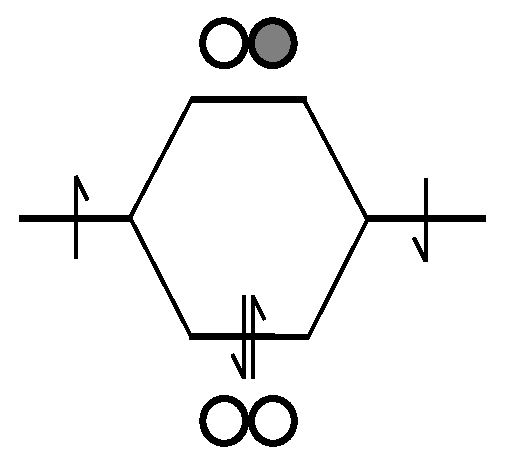
\includegraphics[scale=0.6]{h2-bonding.eps}
\caption{The bonding of two H $1s$ orbitals to make bonding $\sigma_g$
and antibonding $\sigma_u$ orbitals.}
\label{h2-bonding}
\end{center}
\end{figure}

\section{One-Dimensional Periodic Arrays of Atoms}
We already know that the lowest energy state of a hydrogen atom is a
$1s$ orbital. When we bond two hydrogen atoms together we form a
bonding $\sigma_g$ state and an antibonding $\sigma_u$ state; the two
electrons from the H atoms will doubly occupy the $\sigma_g$ state. 
Figure \ref{h2-bonding} shows this interaction.

\begin{figure}
\begin{center}
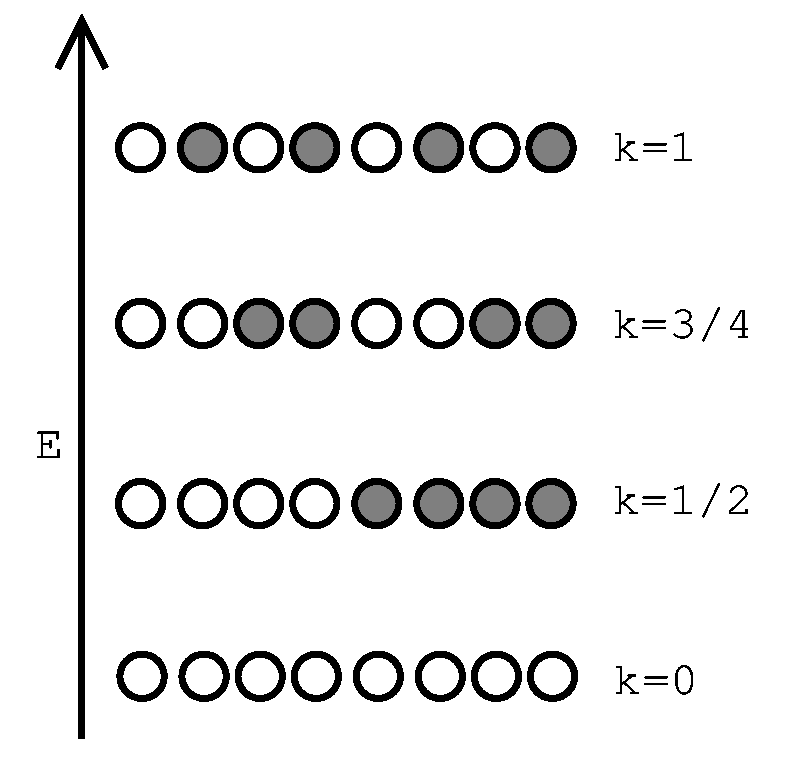
\includegraphics[scale=0.5]{1d-chains.eps}
\caption{Different states that 8 H atoms can have in a one-dimensional
chain, indexed by the $k$-number.}
\label{1d-chains}
\end{center}
\end{figure}

What happens when we take chains of hydrogen atoms? We can think of a
single hydrogen atom as our unit cell that will be translated in one
dimension. Figure \ref{1d-chains} shows different states that eight H
atoms can have. We may approximate the wave function of this system by
\begin{equation}
 \phi(x+X) = \phi_{1s}(x)\cos\left(\frac{2\pi}{a}kx\right).
\label{h-bloch}
\end{equation}
Here $\phi_{1s}$ is the $1s$ wave function for an isolated H atom. $a$
is the lattice spacing between the unit cell images. The
lowercase coordinate $x$ refers to the coordinate within a unit cell,
and the uppercase coordinate $X$ refers to the coordinates between
unit cells. The $k$-number is a measure of how much the phase changes
from one unit cell to the next: when $k=0$ the unit cells are always
replicated with the same sign and when $k=1$ the unit cells alternate
signs. 

\begin{figure}
\begin{center}
\includegraphics[scale=0.5]{1d-EvsK}
\caption{The variation of the energy with the $k$-number for a simple
one-dimensional chain of H atoms.}
\label{1d-EvsK}
\end{center}
\end{figure}

What is remarkable about the $k$-number is that we can boil bonding
configurations, antibonding configurations, and everything in between,
down to a single parameter. We will find it useful to consider the
energy as a function of the $k$-number, as shown in Figure
\ref{1d-EvsK}, which shows how the single energy band varies from the
bonding to the antibonding limit with the variable $k$. 

Since we have one H atom in each unit cell, we only have one electron
in the band, which means that the band will be half-filled: the
$k$-states from 0--1/2 will be occupied, and the $k$-states from
1/2--1 will be unoccupied. Since there is no gap between occupied and
the unoccupied regions, we would predict that this is a metallic
system.

\begin{figure}
\begin{center}
\includegraphics[scale=0.5]{1d-h2-states.eps}
\caption{States of the doubled unit cell with a \chem{H_2} molecule in
each unit cell.}
\label{1d-h2-states}
\end{center}
\end{figure}

\begin{figure}
\begin{center}
\includegraphics[scale=0.5]{1d-h2-bands.eps}
\caption{Band structure of the doubled unit cell with a \chem{H_2}
molecule in each unit cell.}
\label{1d-h2-bands}
\end{center}
\end{figure}

How do we make insulating systems? We can look again at our poly-H
example, but this time we will \emph{double} the unit cell and put a
bonded \chem{H_2} in each cell. The wave function for the valence band
is
\begin{equation}
 \phi_v(x+X) = \sigma_g(x)\cos\left(\frac{2\pi}{a}kx\right),
\label{h2g-bloch}
\end{equation}
and the wave function for the conduction band is
\begin{equation}
 \phi_c(x+X) = \sigma_u(x)\cos\left(\frac{2\pi}{a}kx\right).
\label{h2u-bloch}
\end{equation}
The variation of these states is
shown in Figure \ref{1d-h2-states} and the energy of the resulting
bands is shown in Figure \ref{1d-h2-bands}. Since we now have two
electrons in each unit cell, we can doubly occupy the lower band, and
keep the upper band unoccupied. This configuration leads to an
insulating system, since there is a finite band gap between the
occupied valence band and the unoccupied conduction band.

In the beginning of the chapter when we were describing how single
orbital states were broadened into energy bands we talked about them
being \emph{smeared out}. This simple example shows us that the
process is really much more precise. We can combine the unit cells
with  different translational symmetries, and these different
symmetries have different energies. The $k$-number is a useful way to
index the translational symmetries.

\begin{figure}
\begin{center}
\includegraphics[scale=0.5]{2d-states.eps}
\caption{A two dimensional plane of H atoms with a $k$-state (1,0).}
\label{2d-states}
\end{center}
\end{figure}

The concept of $k$ states is also useful when we have systems that are
periodic in more than one dimension. Figure \ref{2d-states} shows a
two dimensional plane of H atoms, with a $k$-state of (1,0). When we
have a three-dimensional system we specify $(k_x, k_y, k_z)$
states. The next section expands on this idea more.

\section{Reciprocal Space and Brillouin Zones}
The previous system shows that looking at the behavior of the orbital
versus the $k$-vector can give us information about how the entire
energy band works. We can think of the $k$-space $(k_x,k_y,k_z)$
spanned by all possible $k$-vectors as the Fourier transform of the
real $(x,y,z)$ space. This space is known as \emph{reciprocal space}.

The reciprocal space \matvec{d} satisfies
\begin{equation}
 \matvec{b}\cdot\matvec{d}=2\pi.
\end{equation}
These vectors are given by
\begin{equation}
 \matvec{d_j} = \pm2\pi\frac{\matvec{b_k}\times\matvec{b_l}}
                {\matvec{b_1}\cdot(\matvec{b_2}\times\matvec{b_3})}
\end{equation}
where the $+$ sign goes with even permutations of $jkl$, and the $-$
sign goes with odd permutations.

The (first) \emph{Brillouin zone} is the reciprocal space
transform of the unit cell. Just as we will have to integrate over all
points in the unit cell to perform a real space integration, we will
have to integrate over all points in the Brillouin zone to perform a
reciprocal space integration. By understanding the behavior of the
energy bands across the Brillouin zone we may understand all of the
electronic properties of the crystal.

In Figures \ref{1d-EvsK} and \ref{1d-h2-bands} we looked at how the
energy varied with the $k$-state across a band. Unfortunately, for
periodicities higher than 1, we can't put together a simple plot like
this. What we typically do is define \emph{special points} in the
Brillouin zone:
\begin{description} 
\item[$\Gamma$] is defined as (0,0,0); 
\item[X] is defined as (1,0,0); 
\item[K] is defined as (3/4,3/4,0);
\item[W] is defined as (1,1/2,0);
\item[L] is defined as (1/2,1/2,1/2).
\end{description}
We can then describe the variation of the electronic structure of the
entire Brillouin zone by sampling $k$-points that connect these
special points. That is, by sampling the band
structure from $\Gamma$ to $X$ to $W$ to $L$ back to $\Gamma$ to $K$
we can understand the behavior of bands over the entire Brillouin
zone. Figure \ref{si-band} shows such a band structure.

\section{Bloch's Theorem}
The one-dimensional equations \ref{h-bloch}--\ref{h2u-bloch} for the
periodic wave function may be generalized to higher dimensions.
Bloch worked out the solution for the Schrodinger equation in periodic
systems. Bloch proved that solutions of the periodic potential
have the form
\begin{equation}
 \psi(\matvec{k},\matvec{r}) = \mu(\matvec{k},\matvec{r})
    \exp\left(i\frac{2\pi}{a}\matvec{k}\cdot\matvec{r}\right).
\end{equation}
Here the \emph{modulating function} $\mu(\matvec{k},\matvec{r})$ is
the part of the wave function that is the same in every unit cell. The
\emph{phase function} $\exp(i\matvec{k}\cdot\matvec{r})$ multiplies the
modulating function by a wave that has the periodicity of the
crystal. In our simple one-dimensional examples we used a cosine
function, but for mathematical simplicity for real systems we use the
\emph{plane waves} shown here.

\section{Tight Binding Calculations}
\begin{figure}
\begin{center}
\includegraphics[scale=0.5,angle=270]{si_band.eps}
\caption{Band structure of cubic Si using Harrison's tight binding
technique.}
\label{si-band}
\end{center}
\end{figure}

To show an example of how kpoints affect the Hamiltonian in a periodic
calculation, we now discuss a very simple example of such a
calculation. 
Chadi and Cohen \cite{Chadi75} and Harrison \cite{Harrison80} define a
very useful semiempirical technique for doing band calculations on
diamond-like structures such as Si or GaAs. The model Hamiltonian is
defined as:
\begin{equation}
\matvec{H}(\matvec{k})=\left(
\begin{array}{cccccccc}
E_s^c & E_{ss}g_0 & 0 & 0 & 0 & E_{sp}g_1 & E_{sp}g_2 & E_{sp}g_3 \\
E_{ss}g_0 & E_s^a & -E_{sp}g_1^* & -E_{sp}g_2^* & -E_{sp}g_3^* &
  0 & 0 & 0\\
0 & -E_{sp}g_1 & E_p^c & 0 & 0 & E_{xx}g_0 &E_{xy}g_3 &E_{xy}g_2 \\
0 & -E_{sp}g_2 & 0 & E_p^c & 0 & E_{xy}g_3 &E_{xx}g_0 &E_{xy}g_1 \\
0 & -E_{sp}g_3 & 0 & 0 & E_p^c & E_{xy}g_2 &E_{xy}g_1 &E_{xx}g_0 \\
-E_{sp}g_1^* & 0 & E_{xx}g_0^* & E_{xy}g_3^* &E_{xy}g_2^*&
   E_p^a & 0 & 0 \\
-E_{sp}g_2^* & 0 & E_{xy}g_3^* & E_{xx}g_0^* &E_{xy}g_2^*&
   0 & E_p^a & 0 \\
-E_{sp}g_3^* & 0 & E_{xy}g_2^* & E_{xy}g_1^* &E_{xx}g_0^*&
   0 & 0 &E_p^a 
\end{array}
\right)
\label{harrison-ham}
\end{equation}
With the Hamiltonian in this form, one must solve
\begin{equation}
\matvec{H}(\matvec{k})\matvec{c}(\matvec{k}) 
  = E(\matvec{k})\matvec{c}(\matvec{k})
\end{equation}
where the values of \matvec{k} extend over the whole Brillouin zone.
The terms $E_s^c$, $E_{ss}$, $E_{xx}$, $E_{xy}$ are parameters
fit for each different material. The superscript $c$ refers to the
\emph{cation}, that is, the column 3 element in a 3,5 semiconductor,
or the column 2 element in a 2,6 semiconductor; the superscript $a$
refers to the \emph{anion}, the other species in each of these. Of
course, for a pure semiconductor like Si, Si is both the cation and
the anion.

The phase factors $g_0$, $g_1$, $g_2$, $g_3$ determine how the
Hamiltonian changes across the Brillouin zone. These are given by 
\begin{equation}
 g_0(\matvec{k}) = \exp(i\matvec{k}\cdot\matvec{d_1})
    + \exp(i\matvec{k}\cdot\matvec{d_2})
    + \exp(i\matvec{k}\cdot\matvec{d_3})
    + \exp(i\matvec{k}\cdot\matvec{d_4})
\end{equation}
\begin{equation}
 g_1(\matvec{k}) = \exp(i\matvec{k}\cdot\matvec{d_1})
    + \exp(i\matvec{k}\cdot\matvec{d_2})
    - \exp(i\matvec{k}\cdot\matvec{d_3})
    - \exp(i\matvec{k}\cdot\matvec{d_4})
\end{equation}
\begin{equation}
 g_2(\matvec{k}) = \exp(i\matvec{k}\cdot\matvec{d_1})
    - \exp(i\matvec{k}\cdot\matvec{d_2})
    + \exp(i\matvec{k}\cdot\matvec{d_3})
    - \exp(i\matvec{k}\cdot\matvec{d_4})
\end{equation}
\begin{equation}
 g_3(\matvec{k}) = \exp(i\matvec{k}\cdot\matvec{d_1})
    - \exp(i\matvec{k}\cdot\matvec{d_2})
    - \exp(i\matvec{k}\cdot\matvec{d_3})
    + \exp(i\matvec{k}\cdot\matvec{d_4})
\end{equation}
where the lattice vectors for a diamond structure are given by
\begin{equation}
 \matvec{d_1} = (1,1,1)a/4
\end{equation}
\begin{equation}
 \matvec{d_2} = (1,\bar{1},\bar{1})a/4
\end{equation}
\begin{equation}
 \matvec{d_3} = (\bar{1},1,\bar{1})a/4
\end{equation}
\begin{equation}
 \matvec{d_4} = (\bar{1},\bar{1},1)a/4
\end{equation}
and $a$ is the lattice constant.

A sample band structure for Si is shown in Figure \ref{si-band}. In a
tight binding calculation of this type, one performs the following
steps.
\begin{enumerate}
 \item Form the constants $E_s^c$, $E_{ss}$, $E_{xx}$, $E_{xy}$ based 
	on the cation and anion specified in the problem.
 \item For each \emph{kpoint} \matvec{k_i} in the Brillouin zone:
 \begin{enumerate}
   \item Form the Hamiltonian $H(\matvec{k_i})$ from equation
	\ref{harrison-ham}.
   \item Diagonalize the $H(\matvec{k_i})$ and save the energies
	$\{E(\matvec{k_i})\}$.
 \end{enumerate}
 \item Form the band structure by connecting the adjacent points of 
	$\{E(\matvec{k_i})\}$ for all kpoints in the Brillouin zone.
\end{enumerate}

Simple programs to compute tight-binding band structures using this
method are available at 
\href{http://wag.caltech.edu/home/rpm/project/tight-binding}
     {http://wag.caltech.edu/home/rpm/project/tight-binding}.

%\section{Augmented Plane Wave Calculations}

\section{Plane Wave DFT Calculations}
The majority of electronic structure calculations that employ periodic
boundary conditions use density functional theory calculations with
plane waves and pseudopotentials. Several features make plane waves
desirable. Plane waves are already periodic functions, and so they are
a natural choice for use as basis functions on systems that are also
periodic. Furthermore, computing the one- and two-electron integrals
is much easier using plane waves, where most of the integrals are
zero, than any other type of basis function. 

However, several aspects of plane waves make them problematic. The
first is that many more plane wave basis functions are required to
describe an atom than would be required using, for example, Gaussian
basis functions. One can perform a good calculation on water using a
6-31G** basis set with only 25 basis functions. The same level of
accuracy using plane waves requires well over 1000 plane wave
functions. Although, as we already noted, Hamiltonian matrix elements
are much easier to compute using plane waves than using Gaussians, one
still must determine the eigenfunctions of the Hamiltonian, a process
which is time consuming for matrices of this size.

The second problem with plane waves is their inability to describe
local phenomena. Fourier expansions of smooth, delocalized functions
require far fewer plane waves than sharp, localized functions. To keep
the basis set size from getting enormous, plane waves higher than a
certain angular momentum are typically excluded from the basis
set. One of the effects of this exclusion is that plane waves cannot
describe core electrons. Typically this is not a terrible problem,
because \emph{pseudopotentials} (also known as \emph{effective core
potentials}) are typically used to remove the core electrons so that
the plane waves need only describe the valence electrons. However,
this often requires using core potentials for atoms like carbon that
are not always well described with these functions. Nonetheless, in
general the replacement of core electrons with pseudopotentials is an
accurate and a straightforward process. 

However, the inability of plane waves to describe localized phenomena
is potentially a difficulty when describing chemical processes that
might themselves be localized. The bonding of an adatom to a metal
surface will typically be highly localized, and it is not always
practical to add enough basis functions to properly describe
it. Similarly, when PBC code is used to describe finite systems (the
\emph{supercell} method, where the molecule is put in a large enough
unit cell to keep it from seeing its periodic neighbors), rarely are
enough functions used to describe the molecule adequately.

For most solid systems, however, plane waves do an adequate job of
describing the electronic structure.
The next section describes attempts to use localized Gaussian functions in
calculations using periodic boundary conditions to circumvent the
problems plane waves have.

\section{Gaussian Basis Set DFT Calculations}
Techniques using Gaussian basis sets in density functional theory
calculations on systems with periodic boundary conditions are
currently under development. These calculations work by using a
combination of spherically symmetric \emph{reference atoms} to
describe the electron density around each atom. The reference atoms
are defined by specifying a linear combination of Gaussian basis
functions, and must be accurate enough that whatever is omitted is a
slowly varying function. This remainder density may then be described
using a very sparse set of plane wave functions. The SeqQuest program
developed at Sandia National Laboratories with help from the Caltech
Materials and Process Simulation Center uses this approach.

%\section{Example: Diamond and Graphite}

\section{Suggestions for Further Reading}
Kittel's \emph{Introduction to Solid State Physics} \cite{Kittel53}
presents a complete introduction to the field of solid state
physics. Harrison's \emph{Electronic Structure and the Properties of
Solids} \cite{Harrison80} gives a good overview of tight binding
calculations for solids. The classic paper on this method is Slater
and Koster 1954 Physical Review paper \cite{Slater54}. Martin and
Leonard's \emph{Electrons and Crystals} \cite{Martin70} presents a
good general discussion on the electronic properties of solids, but is
regrettably out of print. Thijssen's excellent book
\emph{Computational Physics} \cite{Thijssen99} has a good chapter on
periodic boundary conditions.
